%\chapter{Desarrollo de propuesta de prototipo}\label{cap:capitulo4}

%---------------------------------------------------------------------------
\subsection{Creación de conjunto de datos de entrenamiento y adaptación de nanoGPT}\label{section:Creacion de conjunto de datos} 
Para la propuesta del prototipo objeto de esta investigación se plantea la creación de un conjunto de datos a partir de textos clasificados por categoría de amenazas en internet y de medios digitales. Para ello se tiene una columna de texto plano en formato CSV con contenido sobre la recomendación y una etiqueta de clasificación de la recomendación. Esta columna es procesada por la librería pandas que permite cargar los datos en un dataframe o estructura de datos para el posterior procesamiento.\cite{Reiss2021} \\

\begin{figure}[H]
   \centering % figure is centered on the page
       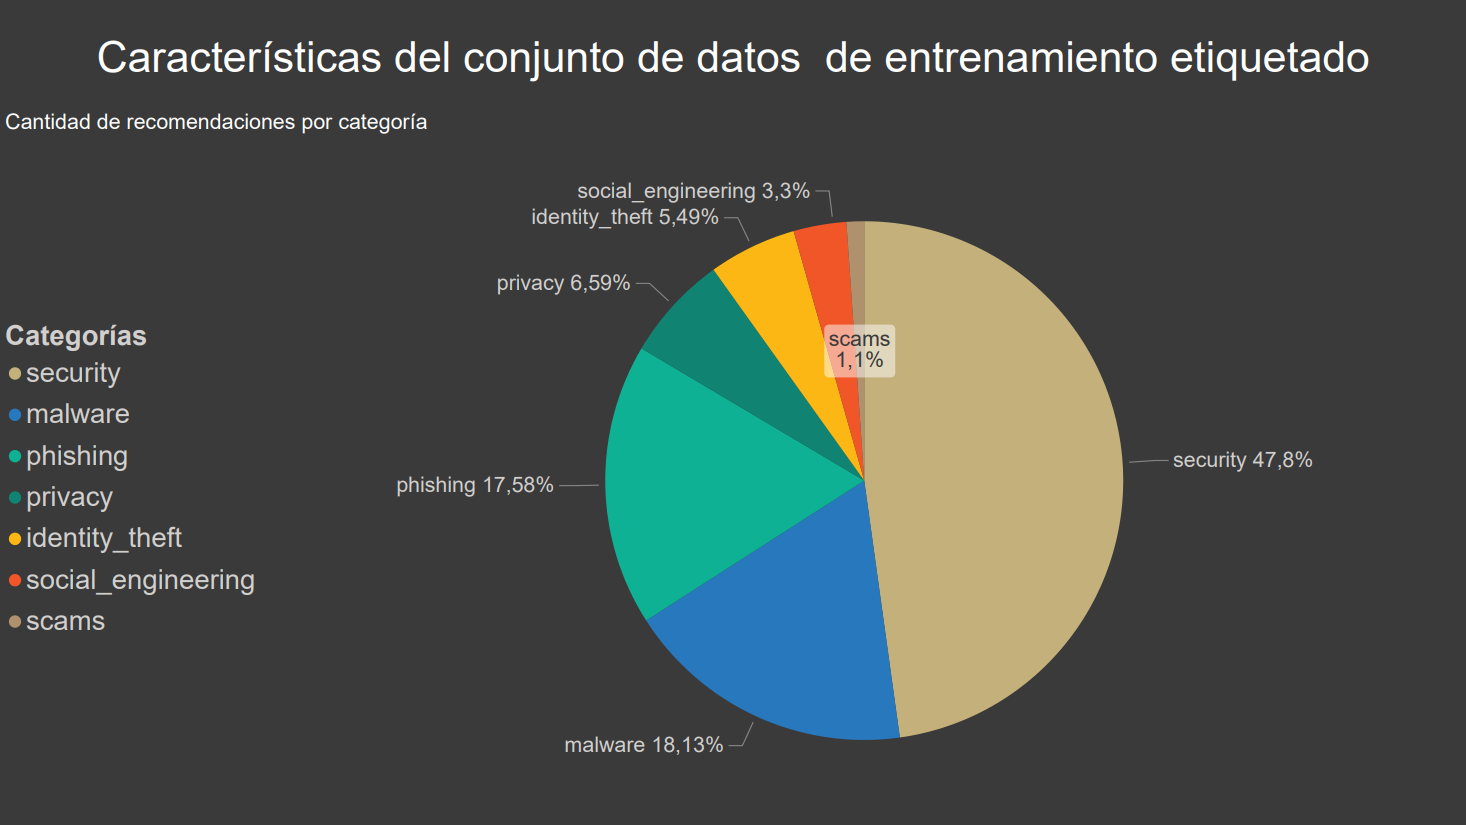
\includegraphics[width=0.7\linewidth]{./doc/Conjunto de datos etiquetado.png} 
   \caption{Características del conjunto de datos etiquetados \cite{}}
  \label{figure:Conjunto de datos}  % assign a unique label to each figure 
\end{figure}
\begin{figure}[H]
   \centering % figure is centered on the page
       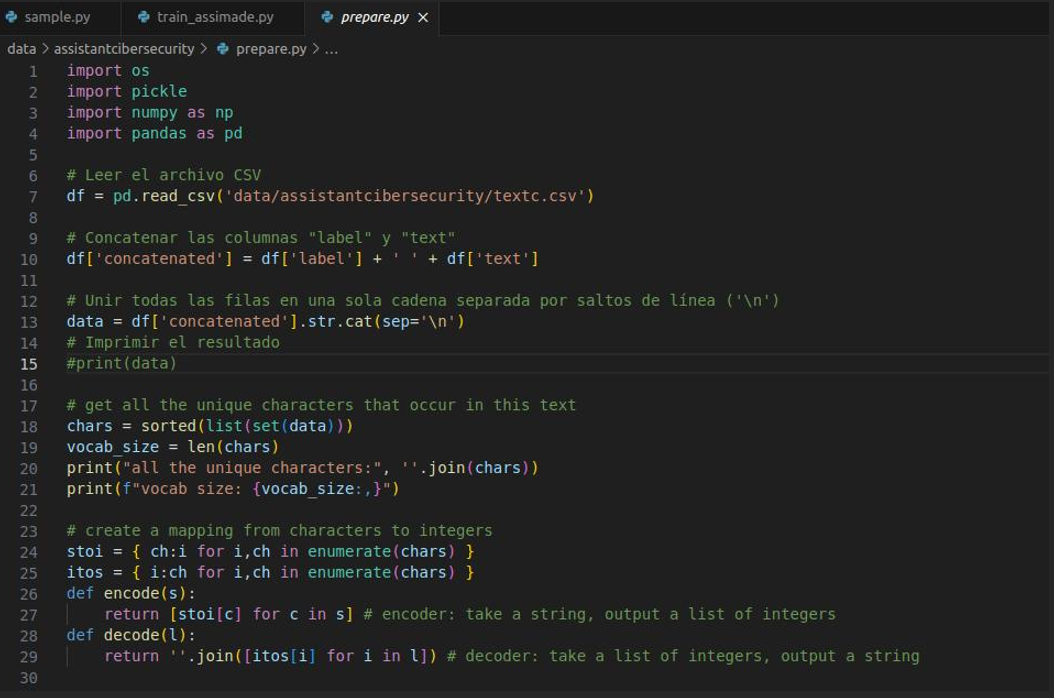
\includegraphics[width=0.8\linewidth]{./doc/02-cr.png} 
   \caption{Configuración para extraer el conjunto de datos en un dataframe y preparación de los datos.  \cite{}}
  \label{figure:Extraxión de datos del csv}  % assign a unique label to each figure 
\end{figure}

Este conjunto de datos es variado y proporciona ejemplos, recomendaciones generales para evitar sesgos de información permitiendo un conjunto de datos de diferentes fuentes para producir resultados más precisos. Para ello se realiza una selectiva elección de datos verdaderos y consistentes.[24] \\
Este conjunto luego se carga para la tokenización, proceso que permite dividir las cadenas en piezas basadas en patrones específicos.[25] El entrenamiento con NanoGPT creando las carpetas que albergan el dataset en formato CSV, luego se procesa para el entrenamiento con iteraciones repetidas. \\

\begin{figure}[H]
   \centering % figure is centered on the page
       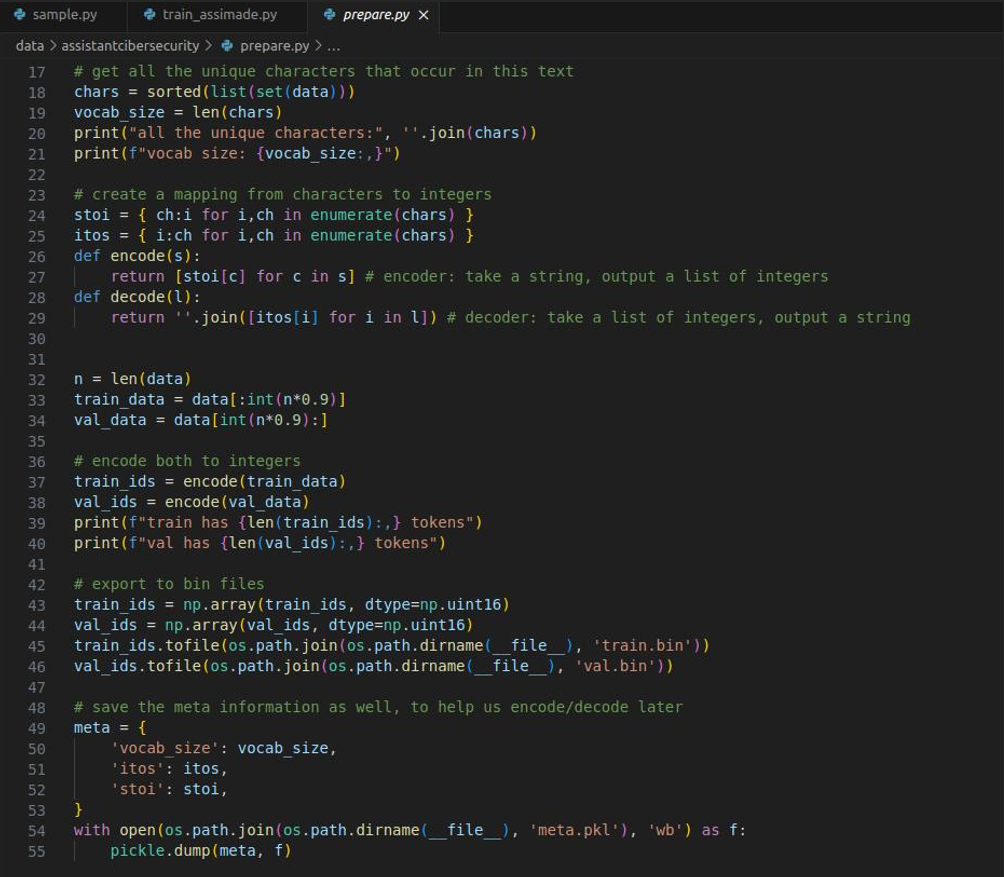
\includegraphics[width=0.8\linewidth]{./doc/03-cr.png} 
   \caption{procesamiento crea  ficheros de validación, entrenamiento y un meta modelo de apoyo.  \cite{}}
  \label{figure:Etapa de encoder}  % assign a unique label to each figure 
\end{figure}
\begin{figure}[H]
   \centering % figure is centered on the page
       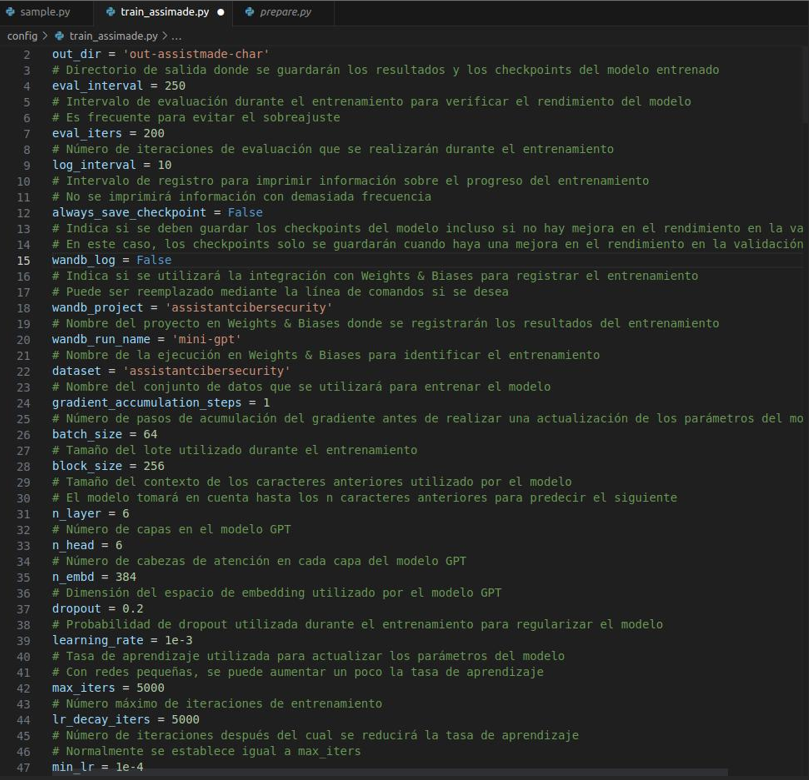
\includegraphics[width=0.8\linewidth]{./doc/04-cr.png} 
   \caption{Configuraciones y parámetros de entrenamiento que crea los directorios de salida para el modelo entrenado.  \cite{}}
  \label{figure:Configuraciónes de parámetros}  % assign a unique label to each figure 
\end{figure}
%---------------------------------------------------------------------------
\subsection{Configuración de los parámetros del código y entrenamiento}\label{figure:Entrenamiento} 
Posteriormente se configuran los parámetros del código para entrenar con los datos un modelo sobre nanoGPT con ciclos de entrenamiento. Para ello se crea finalmente y se evalúan las respuestas y se propone una interfaz para el prototipo con un enfoque MVC.
%-------------------------------------------------------------------------------
\subsubsection{Configuración 1}\label{section:Configuracion1} 
\begin{itemize}
        \item   Objetivo: Ejecutar el entrenamiento de manera más rápida al reducir el número máximo de iteraciones y ajustar otros parámetros.
        \item   Explicación: Esta configuración aumenta el número de capas (n-layer) y cabezas de atención (n-head) a 12 para proporcionar una capacidad de representación más alta. El tamaño del lote (batch-size) se incrementa a 64 para aprovechar mejor los recursos de la CPU. Se reduce el número máximo de iteraciones (max-iters) a 1000 para acelerar el entrenamiento. El número de iteraciones para reducir la tasa de aprendizaje (lr-decay-iters) se establece en 1000. Se mantiene un tamaño de bloque (block-size) de 128 y una dimensión del espacio de embedding (n-embd) de 512 para mantener una representación adecuada del texto. La probabilidad de dropout (dropout) se establece en 0.2 para regularizar el modelo durante el entrenamiento.
    \end{itemize}
    \begin{figure}[H]
   \centering % figure is centered on the page
       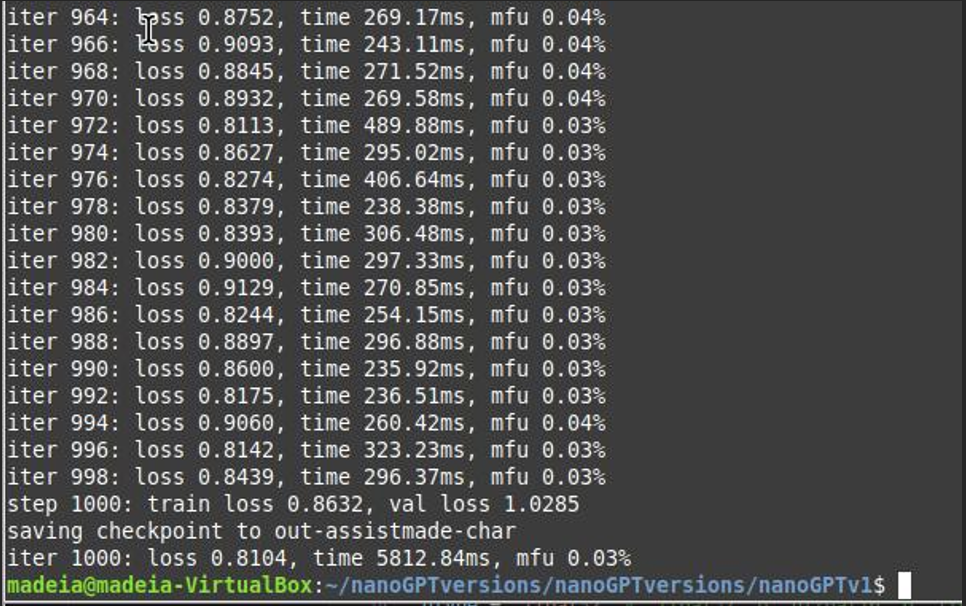
\includegraphics[width=0.65\linewidth]{./rp/15-cp.png} 
   \caption{Proceso de entrenamiento de modelo 1\cite{}}
  \label{figure:Resultado 1}  % assign a unique label to each figure 
\end{figure}
%------------------------------------------------------------------------------
\subsubsection{Configuración 2}\label{section:Configuración de los parámetros del código} 
    \begin{itemize}
        \item   Objetivo: Evaluar el rendimiento y la eficiencia de un modelo ligero en el conjunto de datos proporcionado.
        \item   Explicación: Esta configuración se centra en entrenar un modelo con una arquitectura más simple y menos parámetros para tareas de clasificación en el conjunto de datos de seguridad que permitan acercar. Se utiliza un tamaño de bloque más pequeño (block-size) para limitar el contexto de los caracteres anteriores. 
        \item   Se reduce el número de capas (n-layer) y cabezas de atención (n-head) para disminuir la complejidad del modelo. El tamaño del lote (batch-size) también se reduce para adaptarse a recursos limitados.
    \end{itemize}
\begin{figure}[H]
   \centering % figure is centered on the page
       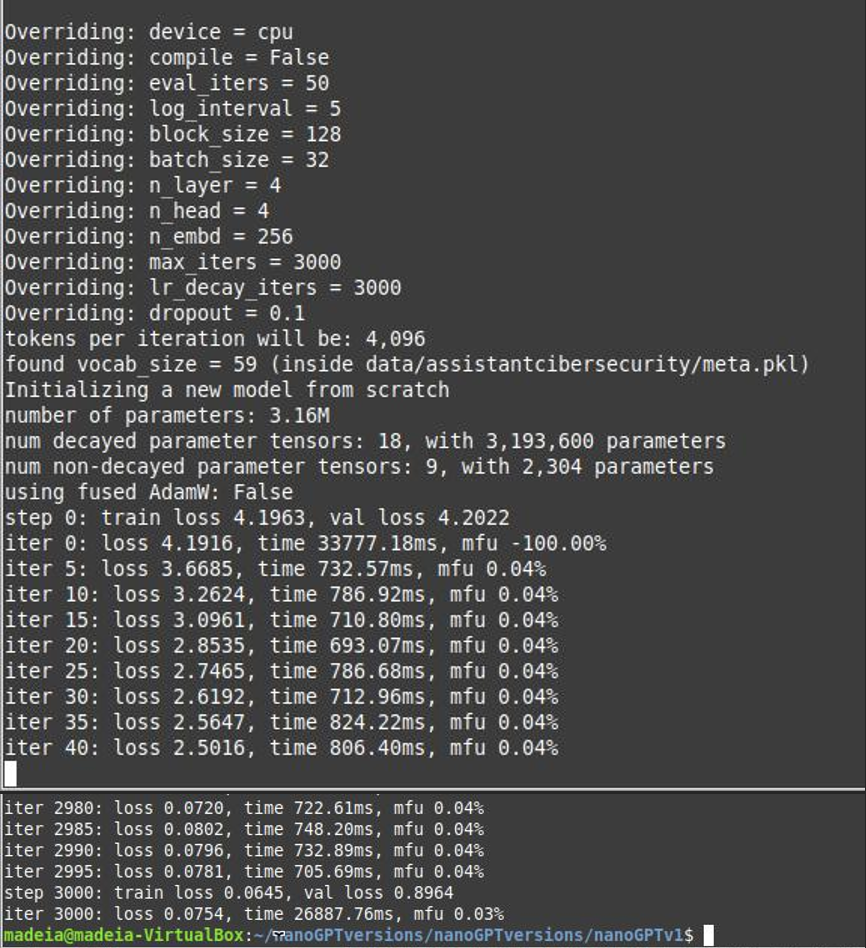
\includegraphics[width=0.65\linewidth]{./rp/05-cp.png} 
   \caption{Configuraciones de entrenamiento de modelo 2  \cite{}}
  \label{figure:Resultado 1}  % assign a unique label to each figure 
\end{figure}
\begin{figure}[H]
   \centering % figure is centered on the page
       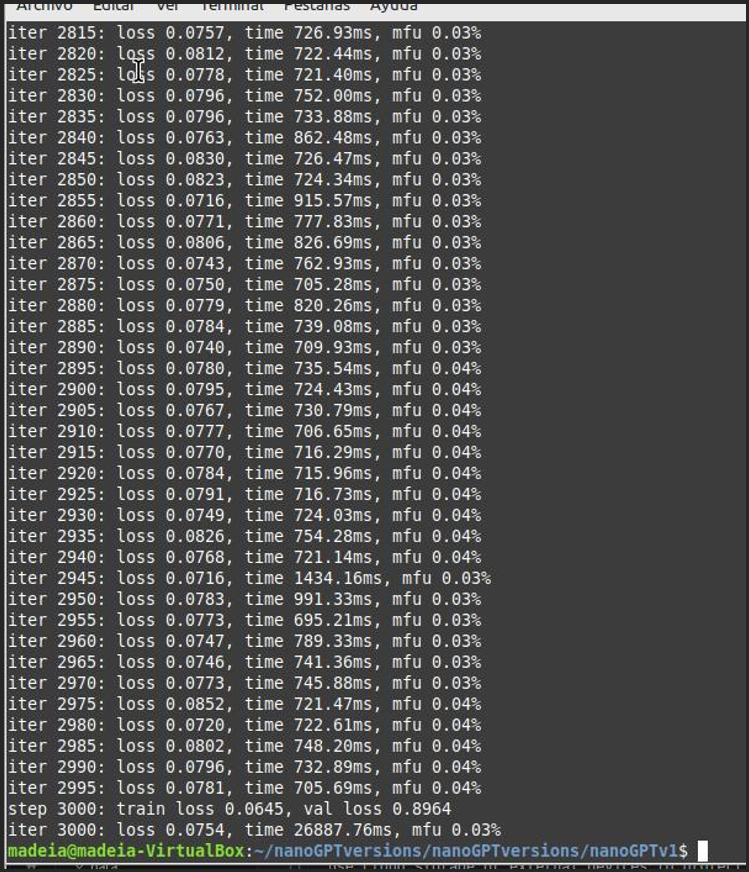
\includegraphics[width=0.65\linewidth]{./rp/06-cp.png} 
   \caption{Proceso de entrenamiento de modelo 2\cite{}}
  \label{figure:Resultado 1}  % assign a unique label to each figure 
\end{figure}
%----------------------------------------------------------------------------
\subsection{Validación del modelo Configuración 1}\label{section:Adaptación de modelo nanoGPT}
\subsubsection{ Prueba 1}\label{section:Adaptación de modelo nanoGPT}
    \begin{itemize}
        \item   Top-k = 100
        \item   Temperatura = 1.2
        \item   Ma-new-tokens = 500
        \item    Prompt = python3 sample.py --out-dir=out-assistmade-char --device=cpu --start=" phising protection tips"
    
\begin{figure}[H]
   \centering % figure is centered on the page
       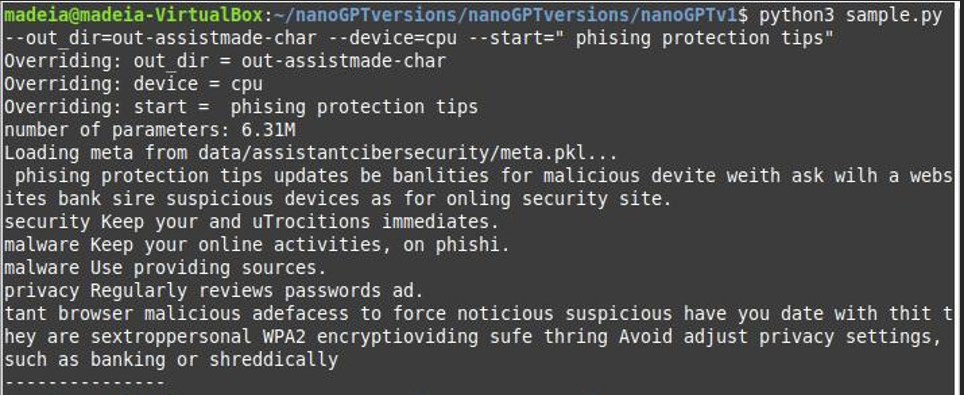
\includegraphics[width=0.65\linewidth]{./rp/16-cp.png} 
   \caption{Resultados de la Prueba 1\cite{}}
  \label{figure:Resultado 1}  % assign a unique label to each figure 
\end{figure}
        \item   Prompt = python3 sample.py --out-dir=out-assistmade-char --device=cpu --start="safe internet browsing "
\begin{figure}[H]
   \centering % figure is centered on the page
       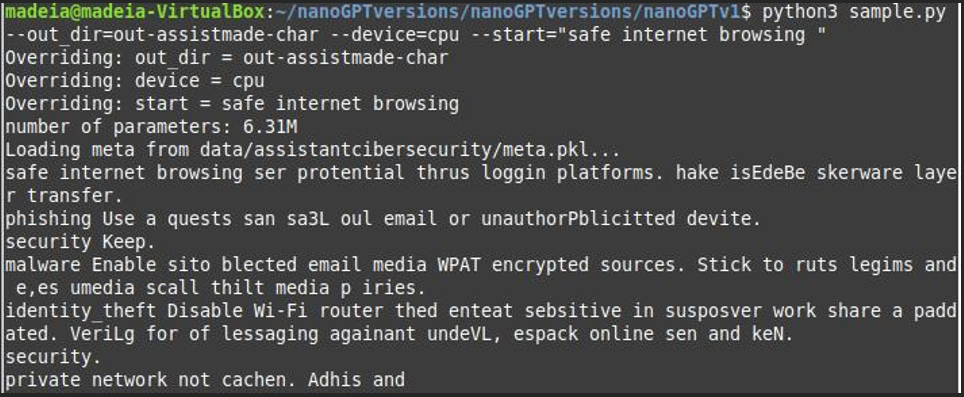
\includegraphics[width=0.65\linewidth]{./rp/17-cp.png} 
   \caption{Resultados de la Prueba 2\cite{}}
  \label{figure:Resultado 1}  % assign a unique label to each figure 
\end{figure}
        \item   Prompt = python3 sample.py –out-dir=out-assistmade-char --device=cpu --start="computer security tips"
\begin{figure}[H]
   \centering % figure is centered on the page
       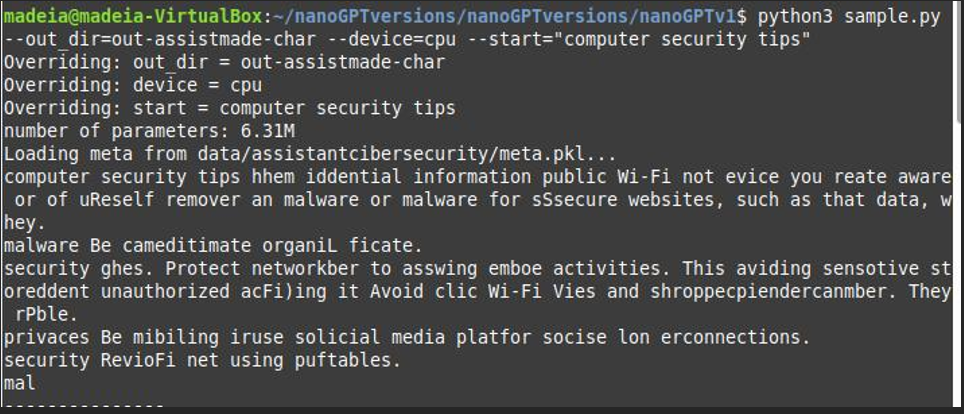
\includegraphics[width=0.65\linewidth]{./rp/18-cp.png} 
   \caption{Resultados de la Prueba 3\cite{}}
  \label{figure:Resultado 1}  % assign a unique label to each figure 
\end{figure}
        \item   Prompt = python3 sample.py --out-dir=out-assistmade-char --device=cpu --start="prevent identity theft"
\begin{figure}[H]
   \centering % figure is centered on the page
       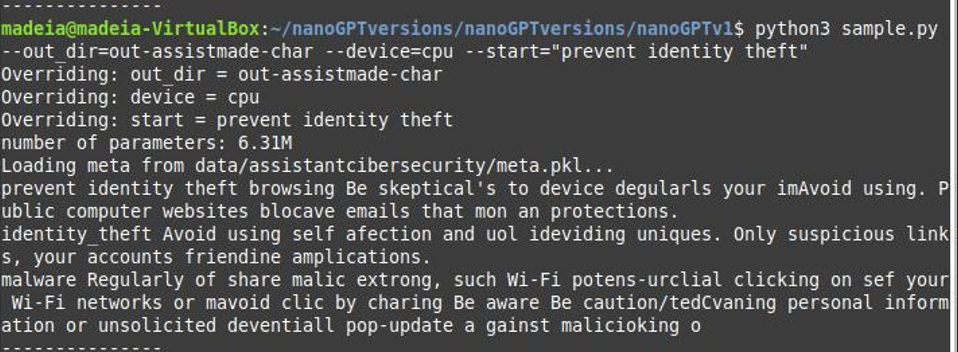
\includegraphics[width=0.65\linewidth]{./rp/19-cp.png} 
   \caption{Resultados de la Prueba 4\cite{}}
  \label{figure:Resultado 1}  % assign a unique label to each figure 
\end{figure}
\end{itemize}
%-----------------------------------------------------------------------------   
\subsection{Validación del modelo Configuración 2}\label{section:Adaptación de modelo nanoGPT}
\subsubsection{ Prueba 1}\label{section:Adaptación de modelo nanoGPT}
    \begin{itemize}
        \item   Top-k = 1
        \item   Temperatura = 10
        \item   Ma-new-tokens = 500
        \item    Prompt = python3 sample.py --out-dir=out-assistmade-char --device=cpu --start=" phising protection tips"
    \end{itemize}
\begin{figure}[H]
   \centering % figure is centered on the page
       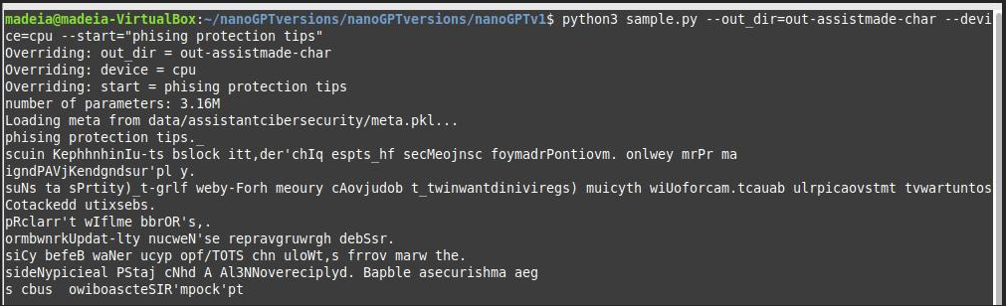
\includegraphics[width=0.65\linewidth]{./rp/07-cp.png} 
   \caption{Resultados de la Prueba 1\cite{}}
  \label{figure:Resultado 1}  % assign a unique label to each figure 
\end{figure}
\subsubsection{ Prueba 2}\label{section:Adaptación de modelo nanoGPT}
    \begin{itemize}
        \item   Top-k = 0.8
        \item   Temperatura = 10
        \item   Ma-new-tokens = 500
        \item   Prompt = python3 sample.py --out-dir=out-assistmade-char --device=cpu --start="safe internet browsing"
    \end{itemize}
\begin{figure}[H]
   \centering % figure is centered on the page
       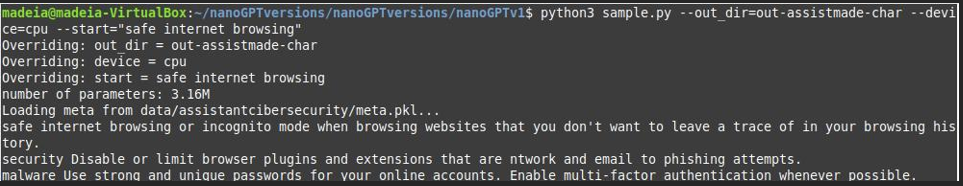
\includegraphics[width=0.65\linewidth]{./rp/08-cp.png} 
   \caption{Resultados de la Prueba 2\cite{}}
  \label{figure:Resultado 1}  % assign a unique label to each figure 
\end{figure}
\subsubsection{ Prueba 3}\label{section:Adaptación de modelo nanoGPT}
    \begin{itemize}
        \item   Top-k = 100
        \item   Temperatura = 1.2
        \item   Ma-new-tokens = 500
            \item   Prompt = python3 sample.py --out-dir=out-assistmade-char --device=cpu --start=" phising protection tips"
            \begin{figure}[H]
              \centering % figure is centered on the page
                  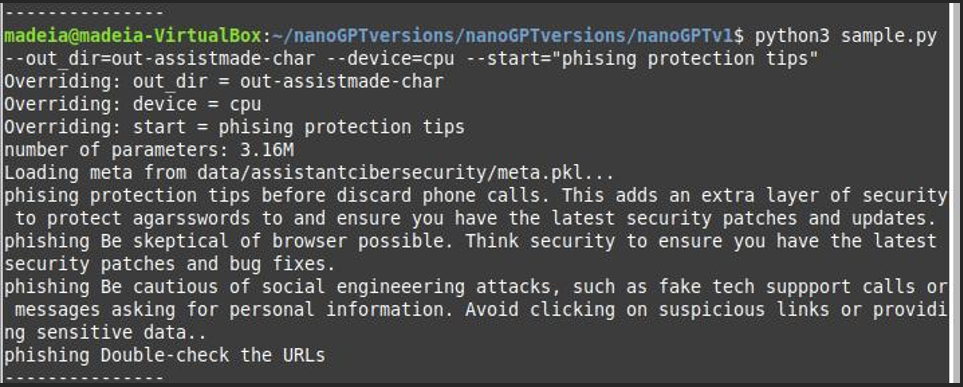
\includegraphics[width=0.65\linewidth]{./rp/09-cp.png} 
              \caption{Resultados de la Prueba 3.1\cite{}}
            \label{figure:Resultado 1}  % assign a unique label to each figure 
            \end{figure}
            \item   Prompt = python3 sample.py --out-dir=out-assistmade-char --device=cpu --start="safe internet browsing"
            \item   Prompt = python3 sample.py --out-dir=out-assistmade-char --device=cpu --start="computer security tips"
            \begin{figure}[H]
              \centering % figure is centered on the page
                  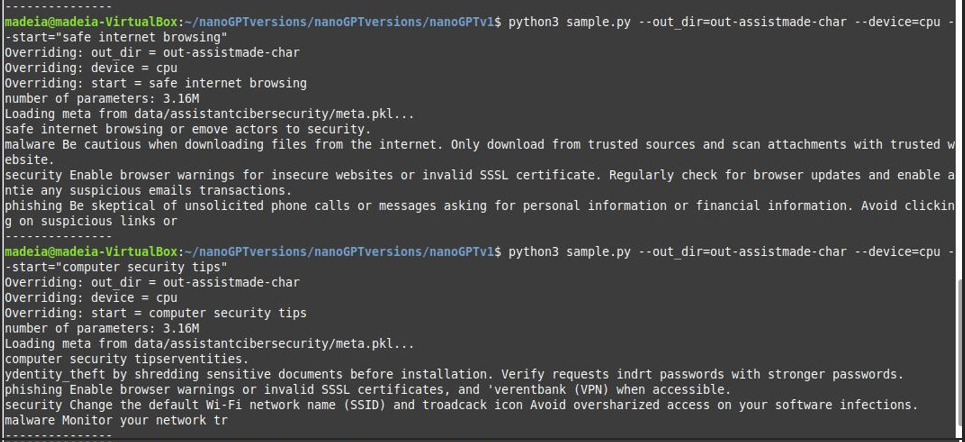
\includegraphics[width=0.65\linewidth]{./rp/10-cp.png} 
              \caption{Resultados de la Prueba 3.2 y 3.3\cite{}}
            \label{figure:Resultado 1}  % assign a unique label to each figure 
            \end{figure}
            \item   Prompt = python3 sample.py --out-dir=out-assistmade-char --device=cpu --start="computer security tips"
            \begin{figure}[H]
              \centering % figure is centered on the page
                  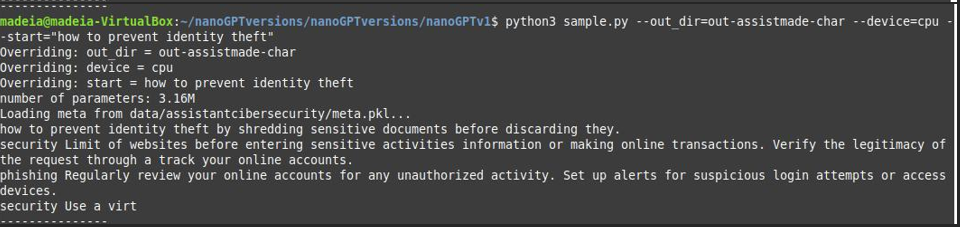
\includegraphics[width=0.65\linewidth]{./rp/11-cp.png} 
              \caption{Resultados de la Prueba 3.4\cite{}}
            \label{figure:Resultado 1}  % assign a unique label to each figure 
            \end{figure}
    \end{itemize}
\subsubsection{ Prueba 4}\label{section:Adaptación de modelo nanoGPT}
    \begin{itemize}
        \item   Top-k = 100
        \item   Temperatura = 1.1
        \item   Ma-new-tokens = 500
            \item   Prompt = python3 sample.py --out-dir=out-assistmade-char --device=cpu --start=" phising protection tips"
            \begin{figure}[H]
              \centering % figure is centered on the page
                  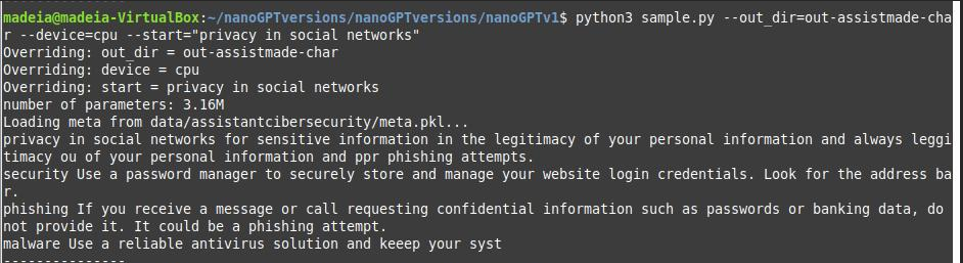
\includegraphics[width=0.65\linewidth]{./rp/12-cp.png} 
              \caption{Resultados de la Prueba 4.1\cite{}}
            \label{figure:Resultado 1}  % assign a unique label to each figure 
            \end{figure}
            \item   Prompt = python3 sample.py --out-dir=out-assistmade-char --device=cpu --start="computer security tips"
            \begin{figure}[H]
              \centering % figure is centered on the page
                  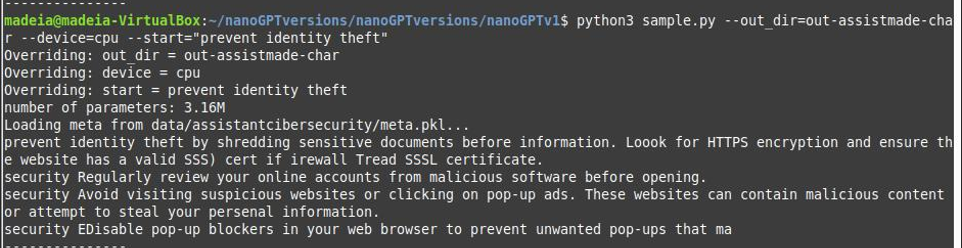
\includegraphics[width=0.65\linewidth]{./rp/13-cp.png} 
              \caption{Resultados de la Prueba 4.2\cite{}}
            \label{figure:Resultado 1}  % assign a unique label to each figure 
            \end{figure}
            \item   Prompt = python3 sample.py --out-dir=out-assistmade-char --device=cpu --start="computer security tips"
            \begin{figure}[H]
              \centering % figure is centered on the page
                  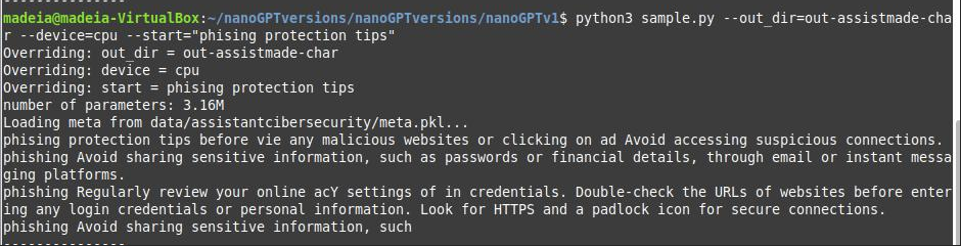
\includegraphics[width=0.65\linewidth]{./rp/14-cp.png} 
              \caption{Resultados de la Prueba 4.3\cite{}}
            \label{figure:Resultado 1}  % assign a unique label to each figure 
            \end{figure}
    \end{itemize}
%---------------------------------------------------------------------------
%------------------------------------------------------------------------------

